\documentclass[a4paper, 12pt, margins=2cm]{homework}
\usepackage{tikz}

\usepackage{graphicx}
\usepackage{dsfont}
\usepackage{microtype}
\usepackage{mathrsfs}
\usepackage[ngerman]{babel}
\usepackage{csquotes}
\usepackage[T1]{fontenc}
\usepackage{lmodern}
\usepackage{wasysym}

\usetikzlibrary{positioning}

\tikzset{main node/.style={circle, fill=black, draw, minimum size=1mm},}

\setlength{\parindent}{0pt}

\newcommand{\R}{\mathbb{R}}
\newcommand{\N}{\mathbb{N}}
\newcommand{\Z}{\mathbb{Z}}
\newcommand{\Q}{\mathbb{Q}}
\newcommand{\C}{\mathbb{C}}

\name{Tobias Eidelpes}
\course{Algebra und Diskrete Mathematik}
\term{2015WS}
\hwnum{6}
\hwtype{Übungsblatt}
\problemtitle{Aufgabe}
\solutiontitle{Lösung}

\begin{document}
  \begin{center}
    \textsc{Beispiele 270, 279, 294, 297, 302, 308, 310}
  \end{center}


% AUSSTÄNDIG
  \problemnumber{270}
  \begin{problem}
    \begin{parts}
      \part \label{270.a}
      In nachstehendem Graphen gebe man je ein Beispiel für
      eine Kantenfolge, die kein Kantenzug ist, einen Kantenzug, der keine Bahn ist,
      bzw. eine Bahn, jeweils vom Knoten 6 zum Knoten 1 an.
      \part \label{270.b}
      Desgleichen finde man eine geschlossene Kantenfolge, die
      kein geschlossener Kantenzug ist, einen geschlossenen Kantenzug, der kein 
      Zyklus ist, bzw. einen Zyklus, jeweils durch den Knoten 5.
      \part \label{270.c}
      Man zeige, dass $G$ schwach, aber nicht stark zusammenhängend ist, und 
      bestimme die starken Zusammenhangskomponenten.
    \end{parts}
    \begin{center}
      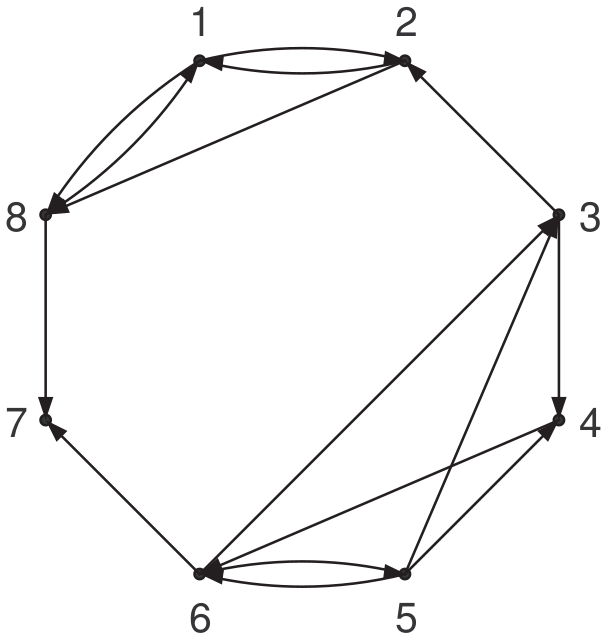
\includegraphics[scale=0.2]{270.png}
    \end{center}
  \end{problem}
  \begin{solution} \hfill

    \ref{270.a}
      Kantenfolge, aber kein Kantenzug (Kanten merhmals verwenden): 
      $$6 \Rightarrow 5 \Rightarrow 6 \Rightarrow 3 \Rightarrow 2 \Rightarrow 1$$
      Kantenzug, aber keine Bahn ()
  \end{solution}


% ERLEDGIGT
  \problemnumber{279}
  \begin{problem}
    Ein schlichter Graph $G = (V, E)$ heißt kubisch, wenn jeder Knoten $v \in V$
    Knotengrad $d(v) = 3$ hat.
    \begin{parts}
      \part \label{279.a}
      Geben Sie ein Beispiel für einen kubischen Graphen mit $\alpha_0(G) = 6$ an!
      \part \label{279.b}
      Gibt es einen kubischen Graphen mit ungerader Knotenanzahl $\alpha_0(G)$?
      \part \label{279.c}
      Zeigen Sie, dass es zu jedem $n \geq 2$ einen kubischen Graphen mit $\alpha_0(G) = 2n$ gibt!
    \end{parts}
  \end{problem}
  \begin{solution} \hfill

      \ref{279.a} \hfill

        \begin{center}
          \def\svgwidth{5cm}
          \input{279.pdf_tex}
        \end{center}

      \ref{279.b} \hfill
        Das Handschlaglemma besagt, dass in jedem Graph die Summe der Grade aller
        Knoten genau doppelt so groß ist wie die Anzahl seiner Kanten:
        \[ \sum_{v\in V(G)}{d(v)} = 2 \cdot |E(G)| \]
        daraus folgt, da bei kubischen Graphen jeder Knoten $v$ den Knotengrad
        $d(v) = 3$ hat, dass die Summe aller Grad die Anzahl der Knoten multipliziert
        mit 3 ist: 
        \[ \sum_{v\in V(G)}{d(v)} = 3 \cdot \alpha_0(G) \]
        \[ 3\cdot \alpha_0(G) = 2\cdot |E(G)| \]
        Da das doppelte der Kantenanzahl immer gerade ist (weil Faktor 2), muss
        die Knotenanzahl auch gerade sein, weil nur eine gerade Zahl mit drei
        multipliziert wieder eine gerade Zahl ergibt. \\

      \ref{279.c} \hfill
        Der Mittelteil des oben gezeichneten Graphen kann beliebig oft hinzugefügt
        werden und man erhält somit zu jedem Graphen einen Graphen mit doppelt so
        vielen Knoten.

  \end{solution}


% AUSSTÄNDIG
  \problemnumber{294}
  \begin{problem}
    Man bestimme im Graphen $G_{10}$ mit Hilfe von $A_{G_{10}}^3$ die Anzahl der
    Dreiecke (d. h. die Anzahl der Kreise der Länge 3).
    \begin{center}
      \def\svgwidth{2.5cm}
      \input{294.pdf_tex}
    \end{center}
  \end{problem}
  \begin{solution}
    \[ \text{Adjazenzmatrix } A_{G_{10}} = \bordermatrix{
      ~ & 1 & 2 & 3 & 4 & 5 \cr
      1 & 0 & 1 & 0 & 1 & 1 \cr
      2 & 1 & 0 & 1 & 0 & 1 \cr
      3 & 0 & 1 & 0 & 1 & 1 \cr
      4 & 1 & 0 & 1 & 0 & 1 \cr
      5 & 1 & 1 & 1 & 1 & 0 
    } \]
  \end{solution}


% AUSSTÄNDIG
  \problemnumber{297}
  \begin{problem}
    
  \end{problem}
  \begin{solution}
    
  \end{solution}


% AUSSTÄNDIG
  \problemnumber{302}
  \begin{problem}
    
  \end{problem}
  \begin{solution}
    
  \end{solution}


% AUSSTÄNDIG
  \problemnumber{308}
  \begin{problem}
    
  \end{problem}
  \begin{solution}
    
  \end{solution}


% AUSSTÄNDIG
  \problemnumber{310}
  \begin{problem}

  \end{problem}
  \begin{solution}
    
  \end{solution}
\end{document}